\chapter{Návrh projektu}
    \section{Cíl projektu}
    Hlavním cílem tohoto projektu je vytvořit modulární a intuitivní stavebnici, která po sestavení umožňuje Ozobotu, nebo Ozobotům jezdit po sestavené dráze.
    
    Snaží se vyřešit fundamentální problém klasického způsobu použití Ozobotů - absolutní statika klasické dráhy po jejím sestavení. Pokud dráhu nakreslíme na papír, stane se statickou, a s žádnými již nakreslenými prvky nemůžeme hýbat. Papír také představuje vedlejší problémy, mezi nimi např. vpití barev při použití fix, po kterém se barvená sekvence může stát pro Ozobota nečitelnou, nebo nekonzistentnost samolepek, na kterých se může Ozobot zaseknout. 
    
    Zároveň se projekt snaží vyřešit problém alternativního přístupu ve formě tabletu, kterým je nedostatek prostoru, zkrátka plocha standardního tabletu je příliš malá na jakékoli normální užívání Ozobota. 
    \section{Architektura}
    Projekt je rozdělen na tři hlavní a jednu vedlejší část: Řídící aplikaci, Ovládací modul, podřízený modul a pasivní prvky.  Každá z těchto částí je nezbytná pro správné fungování dráhy. Projekt je tak sestaven hierarchicky, tedy Řídící aplikace řídí Ovládací modul, který následovně ovládá podřízené moduly (viz obr. \ref{fig:architecture} Schéma architektury.), pro doplnění dráhy jsou použity pasivní prvky.

    Dráha z této stavebnice se skládá na LEGO® desku, a umožňuje tak nekonečné rozšiřování dráhy. Jednotlivé moduly mají vždy dva konektory, aby se k danému modulu dal vždy připojit další. Tyto konektory jsou vzájemně zaměnitelné, tedy \uv{vstupní} se dá použít jako \uv{výstupní} a obráceně (viz obr. \ref{fig:track-design} Schéma sestavené dráhy.).
 \begin{figure}[H]
                \begin{center}
                    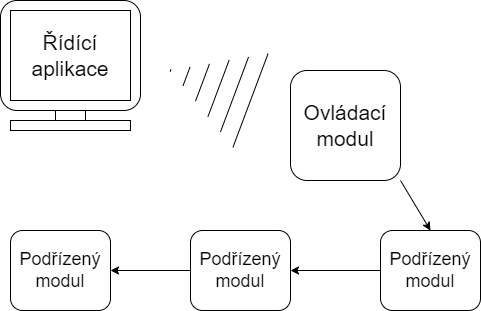
\includegraphics[scale=0.8]{images/schema_architektury.drawio (1).png}
          \caption{Schéma architektury.}
          \label{fig:architecture}
                \end{center}  
        \end{figure}
    \begin{figure}[h!]
          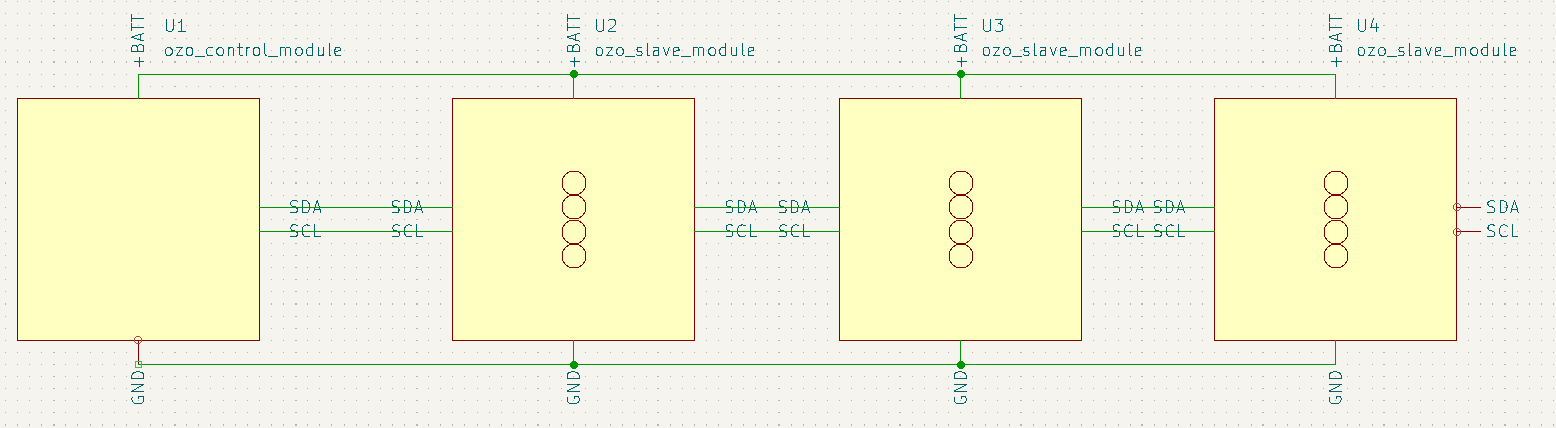
\includegraphics[width=\textwidth]{images/schema_zapojeni.png}
          \caption{Schéma sestavené dráhy.}
          \label{fig:track-design}
        \end{figure}
               
        \newpage
    \section{Řídící aplikace}
        Řídící aplikace slouží ke komunikaci uživatele s celou dráhou, je klíčovým bodem v celkové architektuře. Aplikace je naprogramována ve frameworku .NET, v jazyce C\#, v prostředí WPF.
        
        Aplikace má na starost dvě věci, a to komunikaci s ovládacím modulem, a přijímání dat od uživatele.

        \subsection{Využité technologie}
            \subsubsection{C\#}
            C\#(vyslovuje se "See Sharp") je objektově orientovaný, bezpečně typovaný jazyk vyvinutý společností Microsoft. Patří do rodiny jazyků C a nejvíc se mu podobají jazyky C++, Java a Javascript. Jazyk je součástí .NET Framework a používá se k vývoji různých typů aplikací, jako jsou desktopové aplikace, webové aplikace a mobilní aplikace pro platformy Windows, iOS a Android\cite{CSharp}.
            \subsubsection{.NET}
            .NET je softwarový framework vyvinutý společností Microsoft pro vývoj aplikací na platformě Windows a dalších systémech. Framework zahrnuje soubor nástrojů, knihoven a jazyků pro vývoj, testování a nasazení různých typů aplikací, včetně desktopových aplikací, webových aplikací, mobilních aplikací a her. .NET umožňuje vývojářům psát kód v jazyce C\#, F\# nebo Visual Basic a kompilovat ho do Common Language Runtime (CLR), který běží na operačním systému Windows nebo jiných platformách jako Linux a macOS. Díky .NETu jsou aplikace vytvořené v těchto jazycích škálovatelné, bezpečné a snadno spravovatelné\cite{.NET}.
            \subsubsection{WPF}
            WPF (Windows Presentation Foundation) je součástí .NET Frameworku, který umožňuje vývojářům vytvářet bohaté a interaktivní uživatelské rozhraní pro aplikace běžící na platformě Windows. WPF používá deklarativní jazyk XAML (eXtensible Application Markup Language), který odděluje grafické prvky a prezentaci od kódu aplikace, což umožňuje vývojářům snadněji vytvářet a upravovat uživatelské rozhraní.

            WPF poskytuje řadu pokročilých funkcionálních prvků, jako jsou animace, přechody, efekty, multi-touch ovládání a podpora pro 2D a 3D grafiku, což umožňuje vytvářet moderní a dynamické uživatelské rozhraní. WPF také poskytuje flexibilní a konfigurovatelné datové vazby, které umožňují vývojářům snadno propojovat datové zdroje s uživatelským rozhraním\cite{WPF}.
            
        \subsection{Komunikace s ovládacím modulem}
            Pro komunikaci je ve vizuálním prostředí aplikace určena záložka \uv{Connection}(viz obr.~\ref{fig:connection} Záložka \uv{Connection}). V ní můžeme hledat Bluetooth zařízení v okolí, a následně se k~nim připojit. Aby aplikace mohla používat Bluetooth modul zabudovaný do počítače, využívá balíček 32Feet.

            Po navázání komunikace může aplikace vysílat data ovládacímu modulu. Provádí tak vždy, když uživatel změní vlastnosti některého z podřízených modulů ve vizuální reprezentaci dráhy(viz Řídící aplikace - Přijímání dat od uživatele).

            \begin{figure}[h!]
          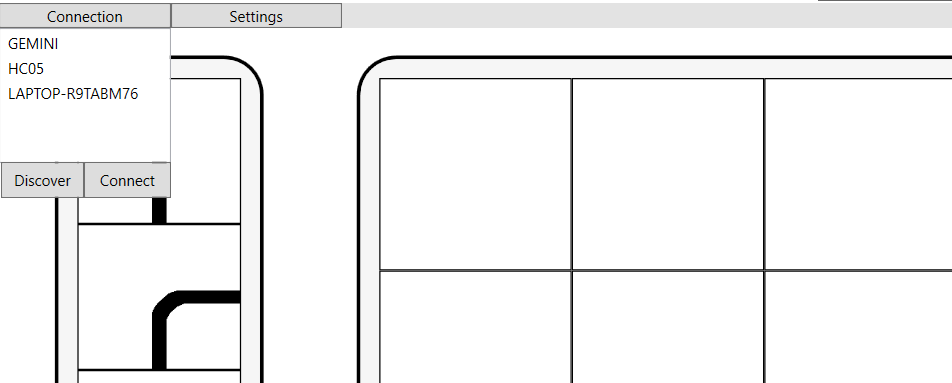
\includegraphics[width=\textwidth]{images/pripojeni.png}
          \caption{Záložka \uv{Connection}.}
          \label{fig:connection}
        \end{figure}
        \begin{figure}[h!]
          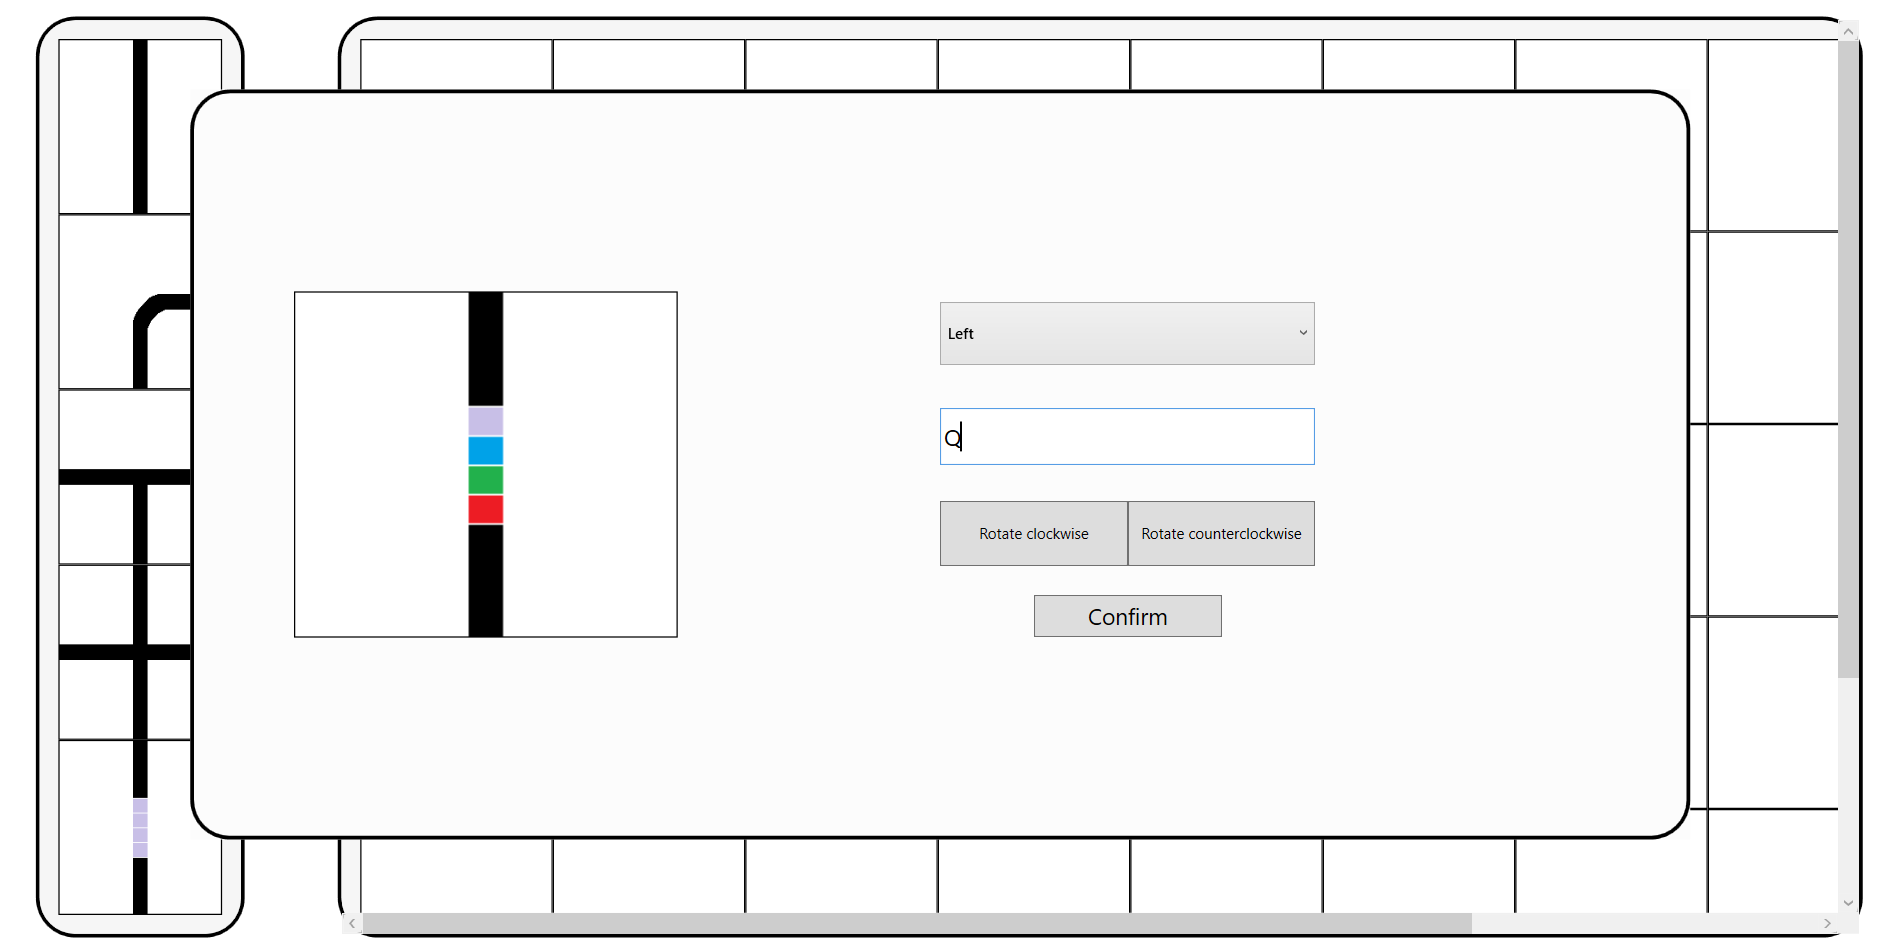
\includegraphics[width=\textwidth]{images/userInput.png}
          \caption{Příjímání dat od uživatele.}
          \label{fig:userInput}
        \end{figure}
        \subsection{Přijímání dat od uživatele}
            Hlavní částí aplikace je vizuální reprezentace dráhy. Jedná se o pole, které může uživatel upravovat tím, že přidává a odebírá jednotlivé bloky dráhy(viz obr. \ref{fig:application} Náhled aplikace - vizuální interpretace dráhy). Na levé straně hlavní plochy jsou na výběr všechny bloky, které se ve stavebnici nacházejí. Uživatel pak může pomocí drag-and-drop systému pokládat jednotlivé bloky na určené místo. Tato funkce umožňuje uživateli naplánovat celou dráhu dopředu, a následně ji sestavit z reálných částí stavebnice.

            Základní velikost pole vizuální reprezentace dráhy je 10 \texttimes~6 bloků. Tato velikost se dá změnit v záložce \uv{Settings}(viz obr. \ref{fig:settings} Záložka \uv{Settings}).

            Po přetažení jednotlivých bloků stavebnice do pole je může uživatel přesouvat z jednoho místa na druhé, a otáčet s nimi. Aktivním prvkům(podřízeným modulům) může upravovat vydávanou barevnou kombinaci. Vždy, když tomu tak učiní, aplikace pošle danou změnu do ovládacího modulu.
            \begin{figure}[h!]
            \begin{center}
          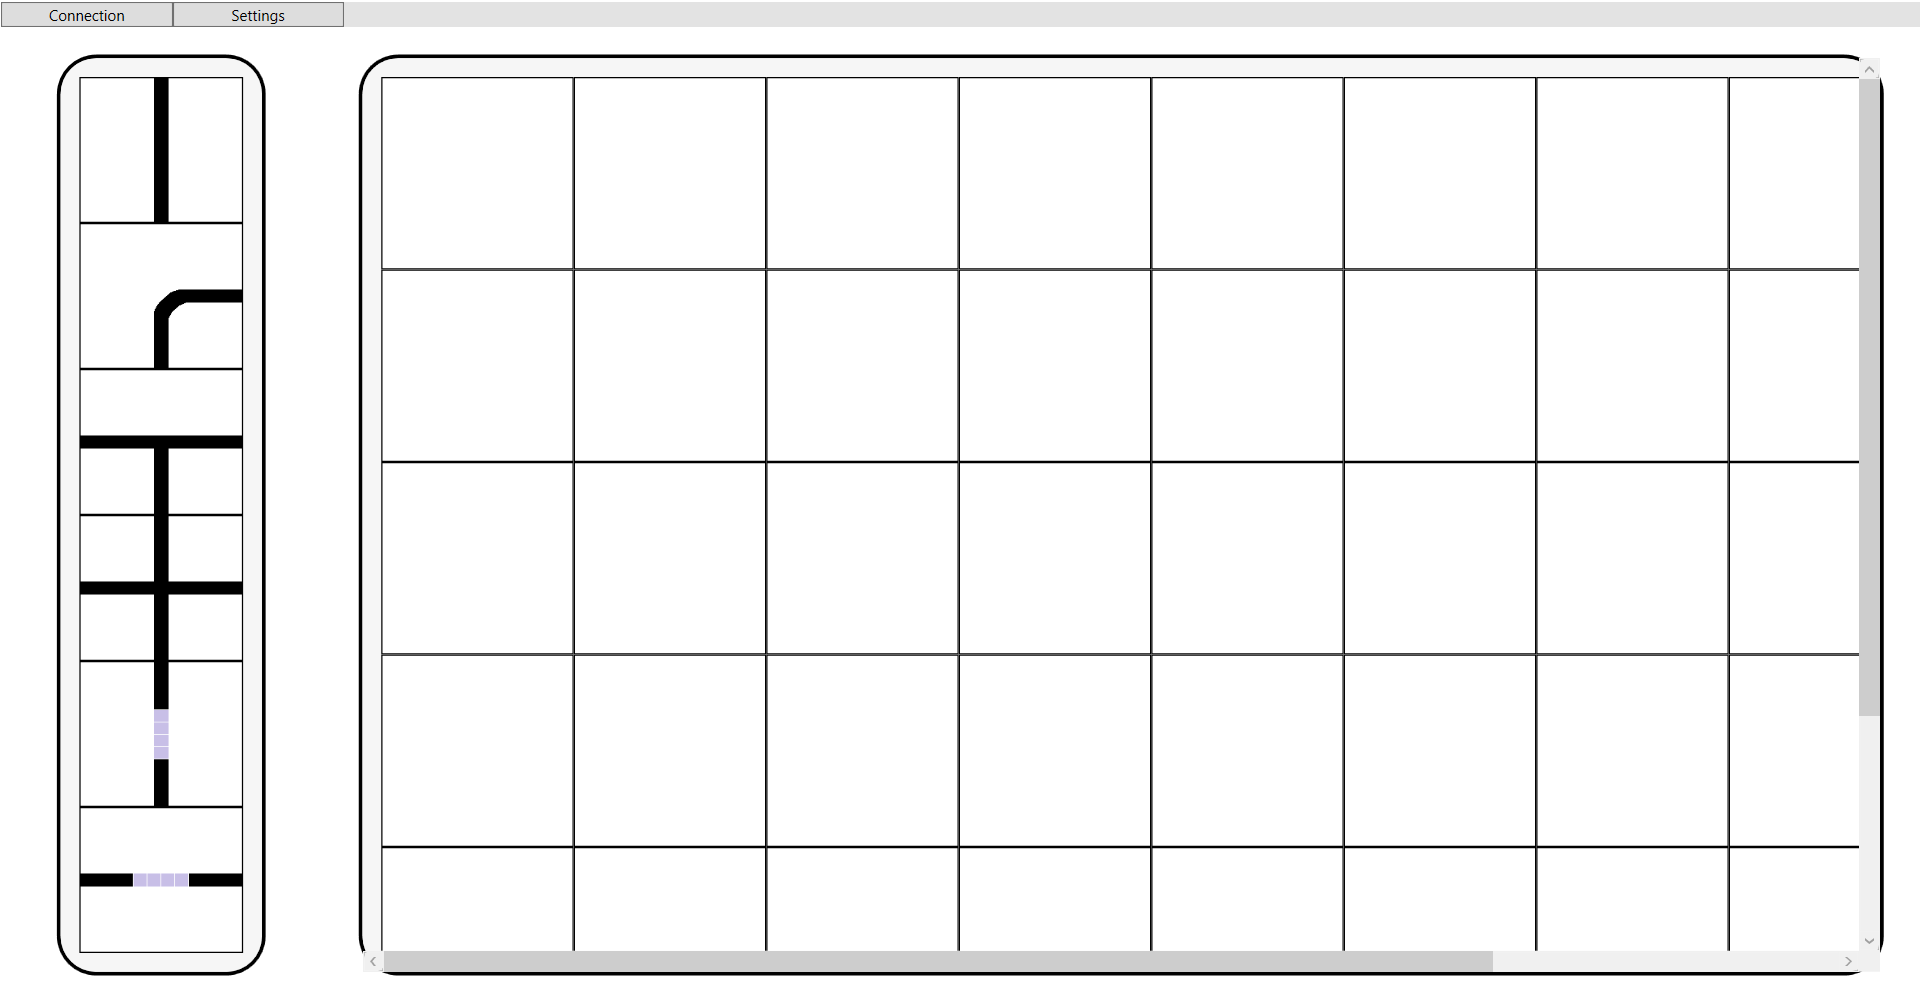
\includegraphics[scale = 0.35]{images/application.png}
          \caption{Náhled aplikace - vizuální reprezentace dráhy.}
          \label{fig:application}
          \end{center}
        \end{figure}
        \begin{figure}[h!]
        \begin{center}
          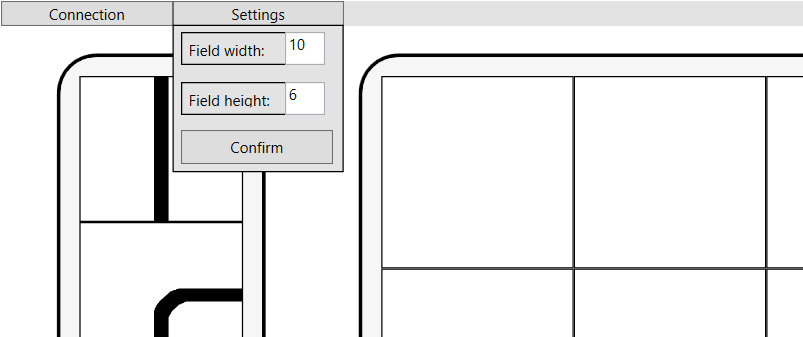
\includegraphics[scale = 0.8]{images/settings.png}
          \caption{Záložka \uv{Settings}.}
          \label{fig:settings}
          \end{center}
        \end{figure}
\newpage
    \section{Ovládací modul}
        Ovládací modul je prostředníkem mezi uživatelem, používajícím řídící aplikaci, a jednotlivými moduly zobrazujícími barevné sekvence. Jeho úkolem je přijímat data z aplikace, tato data zformátovat a poslat na správný podřízený modul ve strukturované podobě. Ovládací modul zároveň slouží jako napájecí zdroj pro celou dráhu.
        \subsection{Fyzické provedení}
        V ovládacím modulu najdeme čtyři hlavní části: baterie s napětím \SI{9}{V}, regulátor napětí, Arduino Nano, a Bluetooth modul (viz\ref{fig:module-design} Schéma zapojení ovládacího modulu.).
        
        Pro veškeré napájení elektřinou je použita alkalická baterie o napětí \SI{9}{V}, jakožto běžně dostupná baterie s napětím větším, než \SI{5}{V} - operačním napětím většiny mikrokontrolérů.
        
        Abychom této elektřiny mohli využít, musí projít regulátorem. V modulu je použit regulátor napětí AMS1117 5.0, který ostatní prvky zásobuje stálým napětím 5V. Tento regulátor potřebuje ke správné funkci napětí alespoň 6,5V, modul bude tedy elektřinou zásoben, dokud je baterie nad touto úrovní napětí.
        
        Mozkem ovládacího modulu je platforma Arduino Nano, disponující mikrokontrolérem ATmega328 a vlastním regulátorem napětí na operačních 5V AMS1117 5.0, který je v~modulu nevyužitý.Platforma Arduino se stará o veškerá data a jejich zpracování.

        Pro komunikaci s řídící aplikací je v ovládacím modulu přítomen Bluetooth modul HC-05 využívající Bluetooth protokol v2.0 s dosahem cca. 10m.

        Veškeré výše zmiňované komponenty jsou uložené v kompaktní schránce z bílého PET plastu. Schránka má velikost podstavy \SI{55.6}{mm} \texttimes~\SI{55.6}{mm} a výšku \SI{53}{mm}. Rozměry podstavy byly vybrány pro kompatibilitu modulu s deskou stavebnice LEGO® a to tak, aby zabírala plochu 7 \texttimes~7 bodů. Tento rozměr je standardem pro všechny moduly, i pasivní prvky. Výška schránky je definovaná především rozměry baterie, která je umístěna v horní části pro její snadnou výměnu.

        \begin{figure}[h!]
          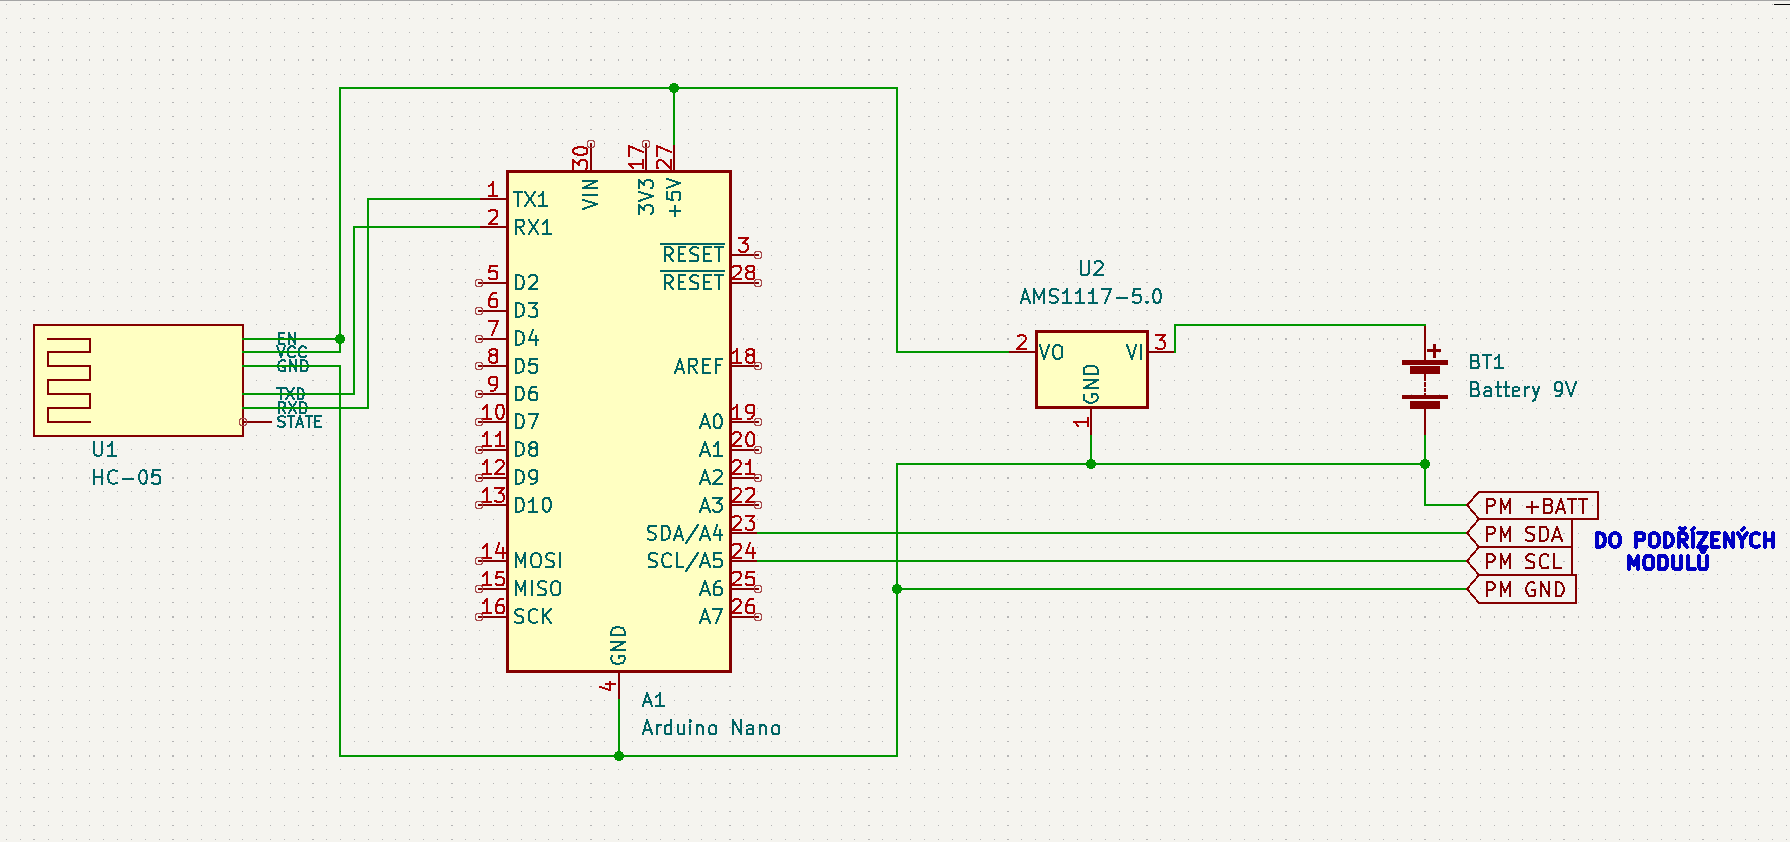
\includegraphics[width=\textwidth]{images/schema_ovladaci.png}
          \caption{Schéma zapojení ovládacího modulu.}
          \label{fig:module-design}
        \end{figure}

        \subsection{Software}
        Modul přijímá data pomocí výše zmiňovaného Bluetooth modulu ve strukturované podobě, a to následovně: Každá instrukce předaná řídící aplikací se skládá ze dvou částí - adresy podřízeného modulu, a samotné barevné kombinace. Pro standardizaci dat na vstupu a výstupu, tedy aby byla každá instrukce vždy pětimístná(první místo pro adresu podřízeného modulu, další čtyři pro jednotlivé diody a jejich barvy), je využito tabulky ASCII. Víme-li tedy adresu podřízeného modulu a správné znaky pro rozsvícení diod (viz obr. \ref{fig:ascii-codes} Tabulka znaků pro kontrolu diod.), můžeme poslat podřízenému modulu instrukci o rozsvícení/zhasnutí barev. 

\begin{figure}[h!]
          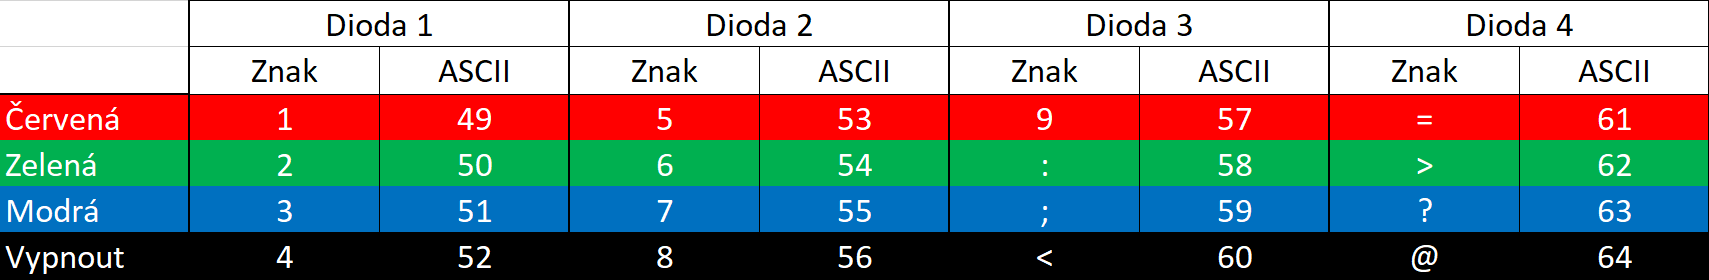
\includegraphics[width=\textwidth]{images/ascii_color_codes.png}
          \caption{Tabulka znaků pro kontrolu diod.}
          \label{fig:ascii-codes}
        \end{figure}

        Předtím, než tato data pošleme jednotlivým modulům, musí být nejdříve rozdělena na instrukce pro jednotlivé diody. Instrukce jsou rozděleny v ovládacím modulu, nikoli v~modulu podřízeném, abychom zbytečně nezatěžovali slabší mikrokontroléry podřízených modulů. Ty pak přebírají \uv{syrové} instrukce, a nejsou tak výpočetně zatížené.

        Ovládací modul tedy převezme pomocí Bluetooth data od řídící aplikace, zjistí z~\uv{hlavičky} těchto dat adresu podřízeného modulu, jednotlivé instrukce rozdělí, dále naváže komunikaci s podřízeným modulem a pošle postupně instrukce o konkrétních diodách a jejich barvách.
        
    \section{Podřízený modul}
        Podřízený modul je hlavní funkční částí Ozodráhy, jedná se o koncový článek, který pomocí barevných sekvencí komunikuje s Ozobotem. Přijímá data od ovládacího modulu a podle nich upravuje chování čtyř RGB LED diod. 
        \subsection{Fyzické provedení}
        Na rozdíl od ovládacího modulu nedisponuje podřízený modul vlastním zdrojem elektřiny. Skládá se ze čtyř hlavních částí: mikrokontroléru, regulátoru napětí, LED diod a schránky, ve které je modul uložen (viz obr. \ref{fig:slave-design} Schéma zapojení podřízeného modulu.).

        Modul disponuje mikrokontrolérem ATtiny826-XU, který byl vybrán z několika důvodů. Jedná se o mikrokontrolér nejnovější řady rodiny čipů AVR, disponuje \SI{8}{kB} Flash paměti a \SI{1}{kB} SRAM, je tedy více než adekvátní pro plnění funkcí ovládacího modulu. Je navíc ideální díky počtu I/O pinů, mezi nimiž jsou dva přímo určené pro komunikaci\cite{ATtiny826}.

        Pro regulátor napětí byl vybrán AMS1117-5.0, který využívá i platforma Arduino. Reguluje poskytovaných \SI{9}{V} z baterie v ovládacím modulu na \SI{5}{V}, což je operační napětí výše zmiňovaného mikrokontroléru.
        
        Čtyři RGB LED diody jsou použity pro samotnou komunikaci s Ozobotem. Jelikož je ale světlo vyzařované z těchto diod moc ostré pro barevný senzor, kterým disponuje Ozobot, každá dioda je připojená přes významně větší rezistor, který snižuje dostupné napětí diody, a tím pádem i intenzitu světla.

        Tyto tři výše zmiňované části jsou usazeny na dvouvrstvý plošný spoj, který má na dvou okrajích konektory pro komunikaci a napájení(viz obr. \ref{fig:pcb-design} Návrh plošného spoje.).

        Stejně jako ovládací modul, i podřízený modul má schránku z bílého PET plastu s tím rozdílem, že schránka pro podřízený modul je navržena tak, aby po její vrchní části mohl jezdit Ozobot. Na ploše vrchní části schránky je tedy proveden výřez, který se v prostřední části prohlubuje, aby skrz tento výřez mohly svítit LED diody. Do tohoto výřezu je zasazen pruh černého PET plastu, který má v prostřední části také řez. Světla z LED diod tedy dosáhnou až na barevný senzor Ozobota, který po tomto černém pruhu jede. Rozměry schránky jsou identické s rozměry schránky ovládacího modulu, tedy 7 \texttimes~7 bodů na desce LEGO®(\SI{55.6}{mm} \texttimes~\SI{55.6}{mm}).
\begin{figure}[H]
        \begin{center}
            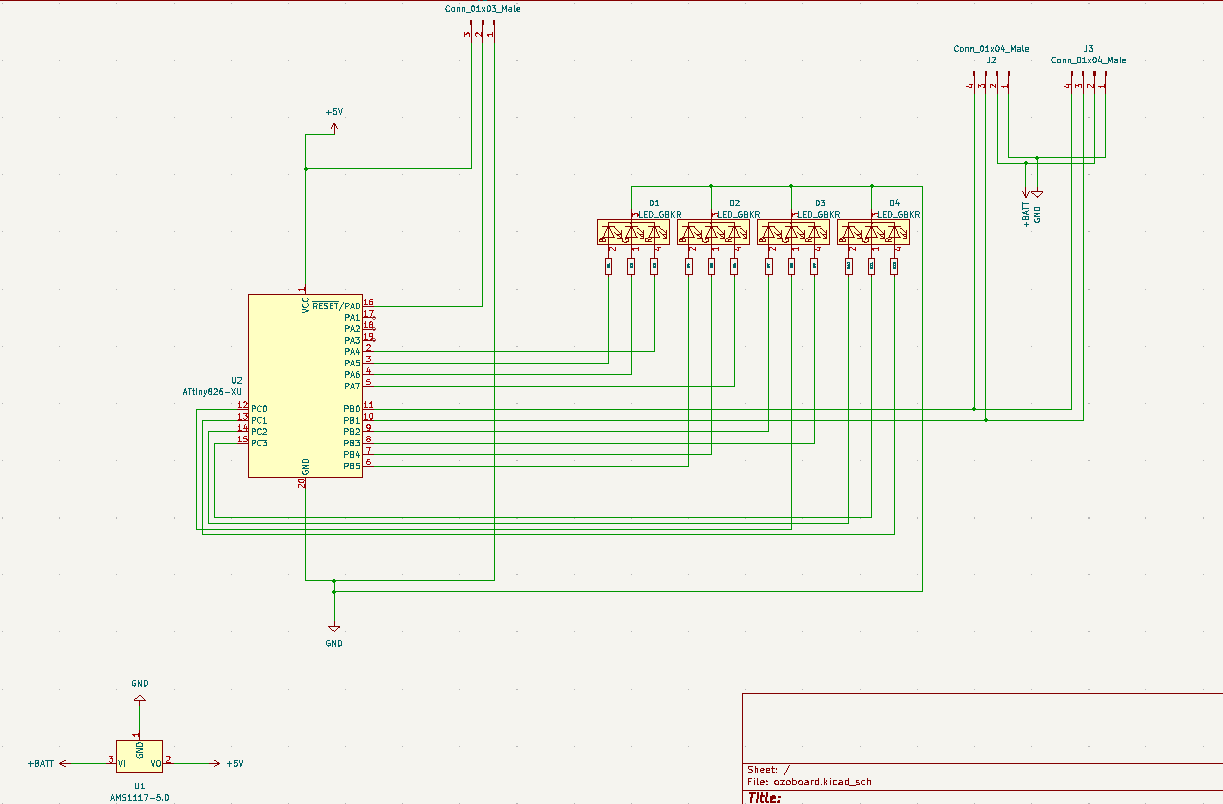
\includegraphics[scale=0.55]{images/schema_podrizeny.png}
          \caption{Schéma zapojení podřízeného modulu.}
        \end{center}      
          \label{fig:slave-design}
        \end{figure}

\begin{figure}[H]
        \begin{center}
          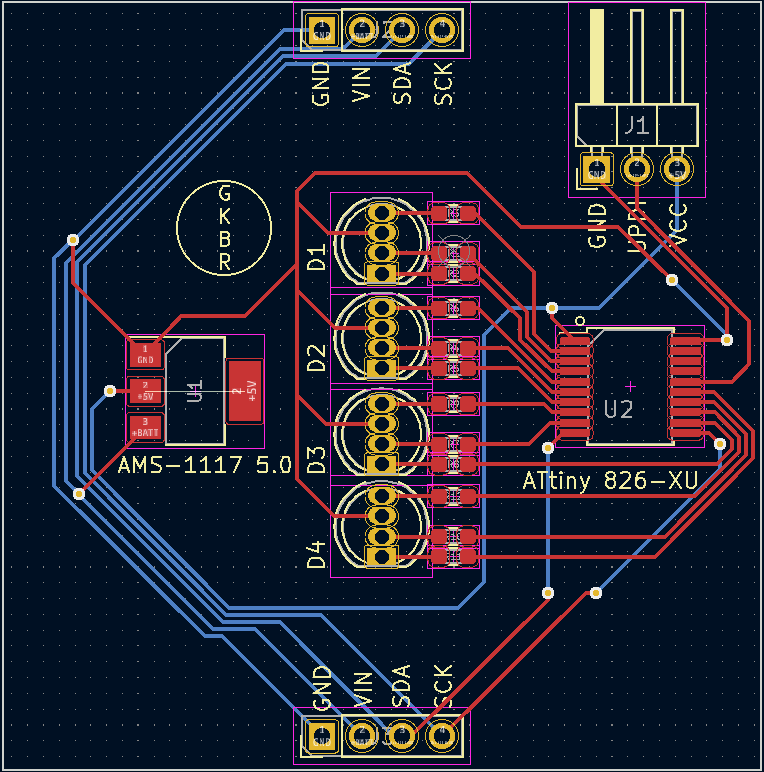
\includegraphics[scale=0.55]{images/navrh_plosny.png}
          \caption{Návrh plošného spoje.}
          \end{center}
          \label{fig:pcb-design}
        \end{figure}

        \subsection{Software}
        Software nahraný na mikrokontrolér musí být dosti kompaktní kvůli omezené paměti mikrokontroléru. Modul přijímá data od ovládacího modulu. Jelikož jsou data strukturována již v ovládacím modulu a podřízený modul přijímá pouze jednotlivé instrukce, složitost programu není veliká. Program pouze přijatá data vyhodnotí podle hodnoty, a rozsvítí/zhasne danou barvu na dané diodě. 

    \section{Pasivní prvky}
        Jelikož ne všechny bloky stavebnice potřebují, nebo dokážou upravovat chování Ozobota (aby Ozobot barvy přečetl, musí jet rovně, zatáčky jsou tedy vyloučeny), stavebnice musí být doplněna o pasivní prvky. Jejich jediným úkolem je vést Ozobota, a nahrazovat tak nakreslenou černou čáru na papíře. Pasivními prvky, neboli bloky jsou: zatáčka, rovný úsek, křižovatka \uv{T} a křižovatka. Tyto bloky mají stejnou šířku a délku jako aktivní prvky(\SI{55,6}{mm} \texttimes~\SI{55,6}{mm}), výšku mají stejnou jako podřízený modul, aby mohl Ozobot přejet z bloků na podřízené moduly bez obtíží, a stavebnice zůstala v jedné rovině. 

        Bloky jsou sestaveny ze dvou částí, a to spodního rámu a plochy pro Ozobota. Obě části jsou vyrobeny z bílého PET plastu. Jelikož se výška podřízeného modulu několikrát během vývoje změnila, bylo zapotřebí vymyslet řešení, aby se při každém vylepšení a následném snížení výšky nemusely všechny bloky vyrábět znovu. Tímto řešením je spodní rám, který může mít libovolnou výšku. Aby byl použitelný, musí ovšem splňovat tři požadavky, a to: kompatibilita s díly LEGO® na spodní straně, kompatibilita s plochou pro Ozobota na vrchní straně a prostor pro protažení kabelů potřebných ke komunikaci mezi ovládacím modulem a podřízenými moduly.

        Plocha pro Ozobota je vrchní část bloku, slouží jako samotná dráha Ozobotu. Stejně jako u podřízeného modulu je v ploše výřez ve tvaru odpovídajícím typu bloku (zatáčka, rovný úsek, křižovatka \uv{T} a křižovatka), do kterého je zasazen pruh černého plastu, nahrazující samotnou černou čáru.

    \section{Komunikace}
            Jedna z nejdůležitějších částí tohoto projektu je komunikace mezi jednotlivými prvky. Rozlišujeme základní dva směry komunikace, a to mezi aplikací a ovládacím modulem, a mezi ovládacím modulem a podřízenými moduly.
        \subsection{Komunikace mezi aplikací a ovládacím modulem}
            Komunikace mezi řídící aplikací a ovládacím modulem je zajištěna technologií Bluetooth, který pro zjednodušení a následné snížení nároků na ovládací modul funguje jednostranně, tedy z řídící aplikace do ovládacího modulu, nikoli opačně. Zařízení s řídící aplikací vysílá data, ovládací modul je pouze přijímá.
            
            Po zapnutí ovládacího modulu se zapne i Bluetooth modul, a čeká na připojení. V řídící aplikaci můžeme následně vyhledat tento Bluetooth modul a navázat s ním spojení.

            Pokaždé, když se v řídící aplikaci změní nastavení některého z ovládacích prvků, tato informace se pošle do ovládacího modulu ve formě stringu. 
        \subsection{Komunikace mezi ovládacím a podřízenými moduly}
            Následná komunikace mezi ovládacím modulem a podřízenými moduly je zajištěna přes variaci protokolu I${^2}$C nazvanou TWI. Jelikož jsou oba mikrokontroléry, jak v ovládacím modulu, tak v podřízeném modulu, z rodiny mikročipů AVR od společnosti Atmel, využívají pro komunikaci stejnou knihovnu \uv{Wire}. 

            
            Ovládací modul přijme data z Bluetooth modulu, tyto data zformátuje a následně naváže komunikaci. Každý podřízený modul má pevně danou adresu, na které přijímá instrukce. Adresový rozsah je momentálně od 65 do 90, reprezentovány v ASCII tabulce znaky \uv{A} až \uv{Z}. Rozsah je zvolen pro přehlednost, a jelikož je počet podřízených modulů momentálně omezen, není důvod ho rozšiřovat. Možnost tento rozsah rozšířit existuje, např od 97 do 122, reprezentováno v ASCII tabulce znaky \uv{a} až \uv{z}.
            
            \textbf{Protokol I${^2}$C}\\
            I${^2}$C protokol je sériový protokol vyvinutý v r.1982 společností Philips. Hojně se používá k řízení OLED a LED displejů v mobilních telefonech, ovládání hlasitosti chytrých reproduktorů, nebo čtení real-time času. Funguje na principu dvou obousměrných linek, jedné pro hodinový signál(SCL) a jedné pro data(SDA).

            Každé vysílání začíná signálem START, kdy je SDA nízká (L) a SCL vysoká (H). Dále následují datové bity, vysílané na lince SDA. Prvních 7 bitů je adresa, osmý je R/W, čili zda chce zařízení psát, nebo číst. Každý byte je ohraničen bitem ACK, který indikuje, zda zařízení odpovídá. ACK bit je vysílán jako H a pokud zařízení odpovídá, přepne v době tohoto bitu SDA na L. Pokud tak neučiní, vysílací zařízení ukončí spojení. Komunikace je ukončena signálem STOP, kdy jsou obě linky vysoké(viz obr. \ref{fig:i2c} I${^2}$C na časové ose.).

            Tento protokol neumožňuje duplexní přenos, vždy může vysílat pouze jedno zařízení, což v případě modulů není problém, jelikož jediný prvek, který vysílá je ovládací modul, podřízený je pouze přijímá na své adrese\cite{i2c}.

            \begin{figure}[H]
                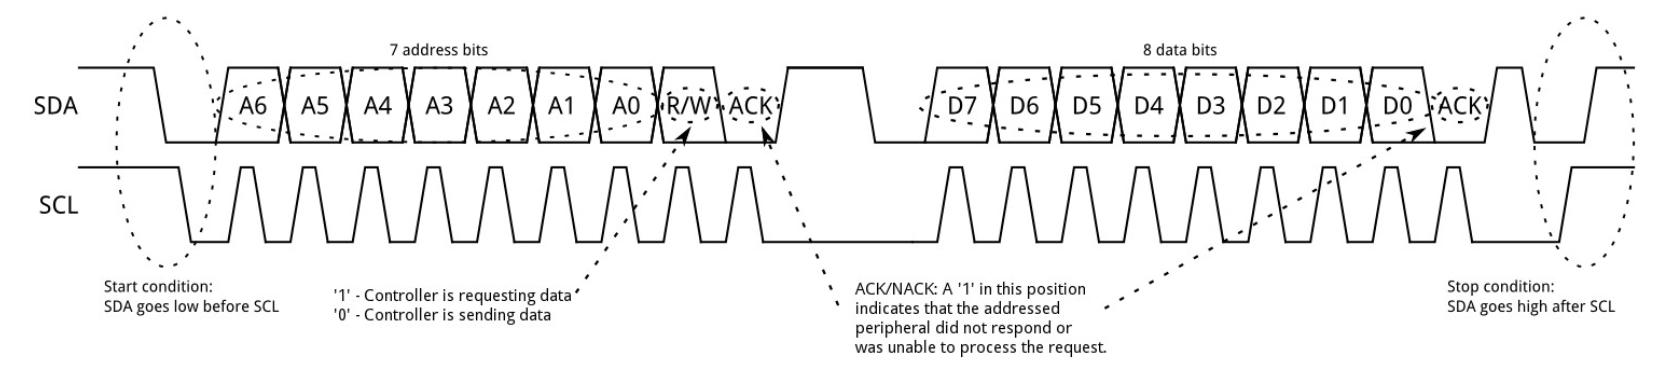
\includegraphics[width=\textwidth]{images/i2c_timing.png}
                \caption{I${^2}$C na časové ose\cite{i2c_graph}.}
                \label{fig:i2c}
            \end{figure}
            \textbf{Protokol TWI}\\
            TWI(Two-Wire Interface) je protokol prakticky identický k I${^2}$C, je kompatibilní s mikrokontroléry společnosti Atmel, mezi nimi i ATmega328 používaný v ovládacím modulu, a ATtiny826 používaný v podřízeném modulu\cite{TWI}.